\documentclass{beamer}
\title{Parallelle Metaheuristieken}
\author{Willem Van Onsem\\Promotor: prof. Bart Demoen}
\date{27 maart 2013}
\usepackage{tikz}
\usetikzlibrary{shapes}
\usepackage[dutch]{babel}
\begin{document}
\begin{frame}
\maketitle
\end{frame}
\begin{frame}
\tableofcontents
\end{frame}
\section{Inleiding}
\section{ParHyFlex}
\begin{frame}{ParHyFlex}
\begin{itemize}
 \item Ontwikkeling van \emph{ParHyFlex}
 \item Parallelle versie van \emph{HyFlex}
 \begin{itemize}
  \item Elke machine houdt een oplossingsruimte bij
  \item Gebruikers ontwikkelen hyperheuristieken
  \item Extra low-level features:
  \begin{itemize}
   \item Afstandsfuncties
   \item Meerdere (virtuele) objectieven
  \end{itemize}
 \end{itemize}
\end{itemize}
\end{frame}
\subsection{Overzicht}
\begin{frame}{ParHyFlex: Structuur}
\begin{figure}
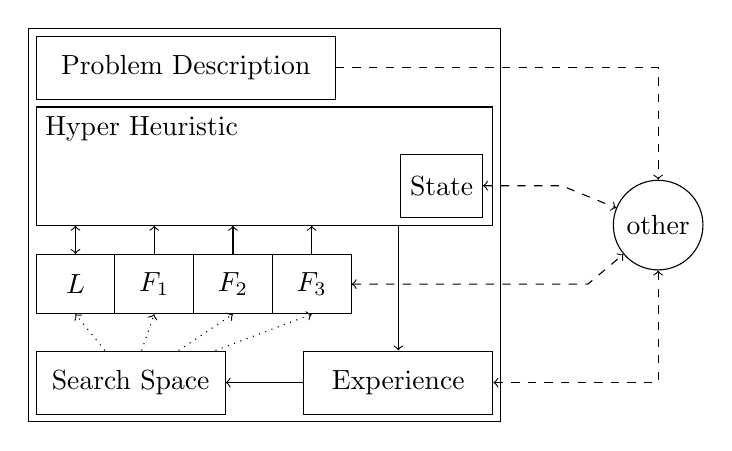
\begin{tikzpicture}
\node[draw,rectangle,minimum width=6cm,minimum height=5cm] (S) at (0,0) {};
\node[draw,rectangle,minimum width=3.8cm,minimum height=0.8cm] (P) at (-1,2) {Problem Description};
\node[draw,rectangle,minimum width=5.8cm,minimum height=1.5cm] (HH) at (0,0.75) {};
\node[draw,rectangle,minimum width=4cm,minimum height=0.75cm] (MEM) at (-0.9,-0.75) {};
\node[draw,rectangle,minimum width=2.4cm,minimum height=0.8cm] (EX) at (1.7,-2) {Experience};
\node[draw,rectangle,minimum width=2.4cm,minimum height=0.8cm] (SS) at (-1.7,-2) {Search Space};
\node[draw,rectangle,minimum width=0.8cm,minimum height=0.8cm] (HHS) at (2.25,0.5) {State};
\node[draw,circle] (O) at (5,0) {other};

\foreach \b in {1,2,3} {
  \draw (\b-2.9,0 |- MEM.north) -- (\b-2.9,0 |- MEM.south);
}

\foreach \b/\t in {0/$L$,1/$F_1$,2/$F_2$,3/$F_3$} {
  \node[minimum width=1cm,minimum height=0.75cm] (M\b) at (\b-2.4,0 |- MEM.east) {\t};
  \draw[dotted,->] (SS) -- (M\b.south);
}

\node[anchor=north west] at (HH.north west) {Hyper Heuristic};

\draw[dashed,->] (P) -| (O);
\draw[dashed,<->] (EX) -| (O);
\draw[dashed,<->] (MEM.east) -- ++(3,0) -- (O);
\draw[dashed,<->] (HHS.east) -- ++(1,0) -- (O);
\draw[->] (HH.south -| EX) -- (EX);
\draw[->] (EX) -- (SS);

\draw[<->] (M0.north) -- (M0 |- HH.south);
\draw[->] (M1.north) -- (M1 |- HH.south);
\draw[->] (M2.north) -- (M2 |- HH.south);
\draw[->] (M3.north) -- (M3 |- HH.south);
\end{tikzpicture}
\caption{Structuur van ParHyFlex}
\end{figure}
\end{frame}
\begin{frame}{ParHyFlex: Structuur}
\emph{Problem Description} component:
\begin{itemize}
 \item Metaprobleem overal gekend
 \item Specifiek probleem aanmaken op \emph{root}
 \item Broadcast naar andere machines
\end{itemize}
\emph{Geheugen} component:
\begin{itemize}
 \item Slaat tussen-oplossingen op
 \item Lokaal lees-schrijf geheugen
 \item Vreemd lees geheugen
 \item Bewaakt door \emph{Search Space}
 \item Met uitwisselingsstrategie (reduceren van bandbreedte)
\end{itemize}
\end{frame}
\begin{frame}{ParHyFlex: Structuur}
\emph{Experience} component:
\begin{itemize}
 \item Vat zoekervaring samen
 \item Wisselt ervaring uit met andere machines
 \item Onderhandelt over nieuwe zoekruimte
 \item Past de actieve zoekruimte aan
 \item Eenheid: \emph{Enforceable Constraints}
 \item Amnesie implementeren
\end{itemize}
\emph{Search Space} component:
\begin{itemize}
 \item Bewaakt de zoekruimte
 \item Past gegenereerde/ontvangen oplossingen aan
 \item Met behulp van \emph{Enforceable Constraints}
 \item Standaard: Positieve set, Negatieve Set
 \item Constraints worden \emph{fuzzy} afgedwongen
\end{itemize}
\end{frame}
\section{Probleem: 3SAT}
\begin{frame}{Probleem: MAX3SAT}
\begin{itemize}
 \item Prestaties framework testen op MAX3SAT
 \item Booleaanse optimalisatie
 \item Motivering:
 \begin{itemize}
  \item Eenvoudig probleem
  \item Veel bestaand onderzoek
  \item Veel aspecten \emph{inherent}
  \item NP-hard (andere problemen omzetten)
 \end{itemize}
\end{itemize}
\end{frame}
\subsection{Componenten}
\begin{frame}{Probleem: MAX3SAT: Componenten}
\emph{Experience} component:
\begin{itemize}
 \item Clause learner
 \item Genereren van clauses die waar zijn voor een oplossing
 \item Evaluatie op andere oplossingen
 \item Variabelen in clause toevallig volgens verdeling
 \begin{equation}
  p(x_i)=(n_i^++n_i^-)\cdot -(p_i^+\log p_i^++p_i^-\log p_i^-)
 \end{equation}
 \item Amnesie: verwijderen van clauses
 \item Merk op: Clause is een \emph{Enforceable Constraint}
 \item Onderhandeling: andere machines plaatsen clauses in negatieve search space, en ervaring set
\end{itemize}
\end{frame}
\subsection{Probleemafhankelijke Componenten}
\section{Communicatie}
\begin{frame}{Communicatie}
\begin{itemize}
 \item Parallelle bibliotheken gericht op computationele problemen
 \item Voorbeeld: Sorteren, Matrix-vermenigvuldiging
 \item Communicatie (aangepaste \emph{TCP})
 \begin{itemize}
  \item Betrouwbaar
  \item Synchroon (\emph{MPI}: optioneel)
  \item Sequenti\"eel (niet bij \emph{Tuple Space})
  \item Atomair
 \end{itemize}
 \item Niet ideaal voor het uitwisselen van oplossingen
 \item Hoge kostprijs (zie verder)
 \item Idee: sommige communicatie over \emph{UDP}
\end{itemize}
\end{frame}
\subsection{Betrouwbaar}
\begin{frame}{Communicatie: Betrouwbaar}
Betrouwbare communicatie?
\begin{itemize}
 \item Parallelle setting: meestal goede verbinding
 \item Geen bewijs dat uitwisseling altijd iets oplevert
 \item Kost van betrouwbaarheid:
 \begin{itemize}
  \item \emph{ACK}-bericht
  \item Heruitsturen (na timeout!)
  \item Netwerk blijft ``outdated berichten sturen''
 \end{itemize}
 \item Voordeel \emph{UDP}:
 \begin{itemize}
  \item Minder bandbreedte
  \item Netwerk als buffer tegen verzadiging
 \end{itemize}
\end{itemize}
\end{frame}
\subsection{Synchroon}
\begin{frame}{Communicatie: Sequentieel}
Synchroon communicatie?
\begin{itemize}
 \item Hyperheuristiek en onderliggende heuristieken divers
 \item Kans om op hetzelfde moment barri\`ere tegen te komen nihiel
 \item Wachten zorgt voor ineffici\"ent CPU-gebruik
 \item Betere strategie: uitsturen en meteen verder werken
 \item ref. \emph{IDP} bevat assynchrone directieven
\end{itemize}
\end{frame}
\subsection{Sequenti\"eel}
\begin{frame}{Communicatie: Sequentieel}
Sequentie\"ele communicatie?
\begin{itemize}
 \item We willen geheugen telkens up-to-date houden
 \item Oplossing uitwisselen indien reeds herzien?
 \item Levert extra bandbreedte op
 \item ref. \emph{Tuple Space} paradigma's
 \item Nadeel: actuelere oplossing niet altijd ``betere''
\end{itemize}
\end{frame}
\subsection{Atomair}
\begin{frame}{Communicatie: Atomair}
Atomaire communicatie?
\begin{itemize}
 \item Diverse communicatie (oplossingen, ervaring, toestand)
 \item Verschillende prioriteiten
 \item Kost van bericht: bericht zelf, aantal bytes minder relevant
 \item Idee: opsparen van berichten en meesturen met anderen
 \item ref. \emph{Piggybacking} van \emph{ACK} in \emph{TCP}
\end{itemize}
\end{frame}
\end{document}
